\documentclass[11pt]{article}

% Mandatory Packages
\usepackage{amsmath}
\usepackage{amssymb}
\usepackage{amsthm}
\usepackage{geometry}
\usepackage{tikz}
\usetikzlibrary{arrows.meta, positioning, shapes}
\usepackage{mathrsfs}
\usepackage{mathtools}
\usepackage{hyperref}
\usepackage{enumitem}

% Geometry Settings
\geometry{a4paper, margin=1in}

% Theorem Environments
\newtheorem{theorem}{Theorem}[section]
\newtheorem{lemma}[theorem]{Lemma}
\newtheorem{proposition}[theorem]{Proposition}
\newtheorem{corollary}[theorem]{Corollary}
\theoremstyle{definition}
\newtheorem{definition}{Definition}[section]
\newtheorem{example}{Example}[section]
\newtheorem{problem}{Problem}

% Title Information
\title{\textbf{Homework 4: Fundamental Properties of Set Operations}}
\author{Tashfeen Omran}
\date{September 2026}

\begin{document}

\maketitle
\tableofcontents
\newpage

\section{Part 1: Comprehensive Introduction, Context, and Prerequisites}

\subsection{Conceptual Introduction: Core Concepts \& Axioms}
In the transition from computational mathematics to advanced abstract mathematics, \textit{set theory} serves as the axiomatic foundation upon which all other structures (topology, probability spaces, algebraic rings) are built. A \textbf{set} is a well-defined collection of distinct objects, considered as an object in its own right. The elements that make up a set can be anything: numbers, functions, random variables, or even other sets.

In this chapter, we analyze the structural operations that allow us to combine and manipulate sets within a universal set $U$:
\begin{itemize}
    \item \textbf{Union ($A \cup B$):} The set of all elements belonging to $A$, or $B$, or both. Defined logically as $\{x \in U \mid x \in A \lor x \in B\}$.
    \item \textbf{Intersection ($A \cap B$):} The set of all elements belonging to both $A$ and $B$. Defined logically as $\{x \in U \mid x \in A \land x \in B\}$.
    \item \textbf{Complement ($\overline{A}$ or $A^c$):} The set of elements in the universal space $U$ that are not in $A$. Defined as $\{x \in U \mid x \notin A\}$.
    \item \textbf{Difference ($A - B$ or $A \setminus B$):} The set of elements in $A$ that are not in $B$. Defined as $\{x \in U \mid x \in A \land x \notin B\}$, which is equivalent to $A \cap \overline{B}$.
\end{itemize}

\subsection{Intuition and Set-Theoretic/Logical Foundations}
The "why" behind set-theoretic theorems fundamentally maps back to the axioms of \textbf{Propositional Logic}. There is a perfect mathematical isomorphism between set operations and logical connectives:
\begin{align*}
    \text{Union } (\cup) &\iff \text{Logical OR } (\lor) \\
    \text{Intersection } (\cap) &\iff \text{Logical AND } (\land) \\
    \text{Complement } (\overline{\phantom{A}}) &\iff \text{Logical NOT } (\neg \text{ or } \sim)
\end{align*}
To prove that two sets $X$ and $Y$ are equal, we cannot merely plug in numbers. We must prove \textbf{mutual inclusion}: $X \subseteq Y$ and $Y \subseteq X$. This technique, often called \textit{element-chasing}, requires taking an arbitrary element $x \in X$, traversing logical deductions to show $x \in Y$, and then proving the reverse.

\subsection{Historical Context and Motivation}
In the late 19th century, Georg Cantor developed \textit{naive set theory}, which allowed sets to be formed by any defined property. In 1901, Bertrand Russell discovered a catastrophic flaw (Russell's Paradox): ``Does the set of all sets that do not contain themselves contain itself?'' This paradox shattered mathematical foundations, forcing mathematicians like Zermelo and Fraenkel to strictly axiomatize set theory (ZFC) to prevent self-referential contradictions. 

Concurrently, in 1933, Andrey Kolmogorov solved the foundational crisis in statistics by using these rigorous set operations to axiomatize Probability Theory. He defined a probability space by mapping abstract random events to sets in a $\sigma$-algebra. Thus, mastering set intersections and complements is strictly equivalent to mastering the conditional probabilities and sample-space partitions used in modern Quantitative Finance and Artificial Intelligence.

\subsection{Key Theorems, Lemmas, and Formulas}
The properties below form a Boolean Algebra for sets. Let $A$, $B$, and $C$ be subsets of a universal set $U$.

\begin{theorem}[Theorem 4.22: Fundamental Laws of Set Operations]
\leavevmode
\begin{enumerate}
    \item \textbf{Commutative Laws:}
    \begin{align*}
        A \cup B &= B \cup A \\
        A \cap B &= B \cap A
    \end{align*}
    \item \textbf{Associative Laws:}
    \begin{align*}
        A \cup (B \cup C) &= (A \cup B) \cup C \\
        A \cap (B \cap C) &= (A \cap B) \cap C
    \end{align*}
    \item \textbf{Distributive Laws:}
    \begin{align*}
        A \cup (B \cap C) &= (A \cup B) \cap (A \cup C) \\
        A \cap (B \cup C) &= (A \cap B) \cup (A \cap C)
    \end{align*}
    \item \textbf{De Morgan's Laws:}
    \begin{align*}
        \overline{A \cup B} &= \overline{A} \cap \overline{B} \\
        \overline{A \cap B} &= \overline{A} \cup \overline{B}
    \end{align*}
\end{enumerate}
\end{theorem}

\subsection{Prerequisites}
\begin{itemize}
    \item \textbf{Propositional Logic:} Mastery of De Morgan's laws for logical statements ($\sim(P \lor Q) \equiv \sim P \land \sim Q$).
    \item \textbf{Direct Proof Techniques:} Familiarity with assuming an arbitrary element belongs to a set without loss of generality.
    \item \textbf{Proof by Cases:} The ability to exhaustively analyze logical bifurcations (e.g., when an element is in a union).
\end{itemize}

\newpage
\section{Part 2: Detailed Homework Solutions}

\textit{Note on Strategic Problem Selection: As per advanced academic directives, I have applied a strategic filter to Section 4.5. Instead of redundant computation, I have selected 6 problems (Problems 4.53, 4.54, 4.55, 4.57, 4.58, 4.59) that span every distinct conceptual archetype (element-chasing mutual inclusion, set difference manipulations, and algebraic substitutions) ensuring robust mastery with maximal efficiency.}

\begin{problem}[4.53]
Prove that $A \cap (B \cup C) = (A \cap B) \cup (A \cap C)$ for every three sets $A$, $B$, and $C$ (Theorem 4.22(3b)).
\end{problem}
\begin{proof}[Proof by Mutual Inclusion]
\textbf{Part 1: Show $A \cap (B \cup C) \subseteq (A \cap B) \cup (A \cap C)$.} \\
Let $x \in A \cap (B \cup C)$ be an arbitrary element. By the definition of set intersection, we know two facts simultaneously: $x \in A$, and $x \in B \cup C$.
By the definition of set union, the statement $x \in B \cup C$ implies that $x \in B$ or $x \in C$. We now proceed by cases based on this disjunction. \\
\textit{Case 1: Suppose $x \in B$.} Since we have established $x \in A$ and $x \in B$, it follows by definition of intersection that $x \in A \cap B$. By definition of union, since $x \in A \cap B$, it trivially follows that $x \in (A \cap B) \cup (A \cap C)$. \\
\textit{Case 2: Suppose $x \in C$.} Since we have established $x \in A$ and $x \in C$, it follows that $x \in A \cap C$. Therefore, $x \in (A \cap B) \cup (A \cap C)$. \\
In both exhaustive cases, $x \in (A \cap B) \cup (A \cap C)$. Thus, the forward subset inclusion holds.

\vspace{2mm}
\noindent\textbf{Part 2: Show $(A \cap B) \cup (A \cap C) \subseteq A \cap (B \cup C)$.} \\
Let $x \in (A \cap B) \cup (A \cap C)$. By definition of set union, we have $x \in A \cap B$ or $x \in A \cap C$. We again analyze the exhaustive cases. \\
\textit{Case 1: Suppose $x \in A \cap B$.} By definition of intersection, this implies $x \in A$ and $x \in B$. Because $x \in B$, the definition of union allows us to assert that $x \in B \cup C$. Since we have both $x \in A$ and $x \in B \cup C$, by definition of intersection, $x \in A \cap (B \cup C)$. \\
\textit{Case 2: Suppose $x \in A \cap C$.} This implies $x \in A$ and $x \in C$. Because $x \in C$, we can assert $x \in B \cup C$. Because $x \in A$ and $x \in B \cup C$, it follows that $x \in A \cap (B \cup C)$. \\
Since both cases lead to the same conclusion, the reverse inclusion holds.

Since $A \cap (B \cup C) \subseteq (A \cap B) \cup (A \cap C)$ and $(A \cap B) \cup (A \cap C) \subseteq A \cap (B \cup C)$, the sets are strictly equal.
\end{proof}

\begin{problem}[4.54]
Prove that $\overline{A \cap B} = \overline{A} \cup \overline{B}$ for every two sets $A$ and $B$ (Theorem 4.22(4b)).
\end{problem}
\begin{proof}[Proof by Mutual Inclusion]
\textbf{Part 1: Show $\overline{A \cap B} \subseteq \overline{A} \cup \overline{B}$.} \\
Let $x \in \overline{A \cap B}$. By the definition of the complement operator, $x \notin A \cap B$. 
This means that the logical statement ``$x \in A$ and $x \in B$'' is false. Applying De Morgan's Law for propositional logic ($\sim(P \land Q) \equiv \sim P \lor \sim Q$), we deduce that $x \notin A$ or $x \notin B$. 
By definition of set complement, this translates to $x \in \overline{A}$ or $x \in \overline{B}$. 
By definition of set union, $x \in \overline{A} \cup \overline{B}$. This establishes the forward inclusion.

\vspace{2mm}
\noindent\textbf{Part 2: Show $\overline{A} \cup \overline{B} \subseteq \overline{A \cap B}$.} \\
Let $x \in \overline{A} \cup \overline{B}$. By definition of union, $x \in \overline{A}$ or $x \in \overline{B}$.
By definition of set complement, $x \notin A$ or $x \notin B$. 
Therefore, it cannot be true that $x$ is simultaneously an element of both $A$ and $B$. 
Consequently, $x \notin A \cap B$. 
By definition of the set complement, $x \in \overline{A \cap B}$. This establishes the reverse inclusion.

Since mutual inclusion is proven, $\overline{A \cap B} = \overline{A} \cup \overline{B}$.
\end{proof}

\begin{problem}[4.55]
Let $A, B$, and $C$ be sets. Prove that $(A - B) \cap (A - C) = A - (B \cup C)$.
\end{problem}
\begin{proof}[Proof by Mutual Inclusion]
\textbf{Part 1: Show $(A - B) \cap (A - C) \subseteq A - (B \cup C)$.} \\
Let $x \in (A - B) \cap (A - C)$. By definition of intersection, $x \in A - B$ and $x \in A - C$. 
By definition of set difference, $x \in A - B$ implies $x \in A$ and $x \notin B$. 
Similarly, $x \in A - C$ implies $x \in A$ and $x \notin C$. 
Consolidating these facts, we know that $x \in A$, and simultaneously $x \notin B$ and $x \notin C$. 
By De Morgan's Laws for logic ($\sim P \land \sim Q \equiv \sim(P \lor Q)$), the condition that $x$ is neither in $B$ nor in $C$ means that $x \notin B \cup C$. 
Since $x \in A$ and $x \notin B \cup C$, by definition of set difference, $x \in A - (B \cup C)$.

\vspace{2mm}
\noindent\textbf{Part 2: Show $A - (B \cup C) \subseteq (A - B) \cap (A - C)$.} \\
Let $x \in A - (B \cup C)$. By definition of set difference, $x \in A$ and $x \notin B \cup C$. 
The statement $x \notin B \cup C$ means it is false that $x \in B$ or $x \in C$. 
By logical negation, this means $x \notin B$ and $x \notin C$. 
Since $x \in A$ and $x \notin B$, we have $x \in A - B$. 
Since $x \in A$ and $x \notin C$, we have $x \in A - C$. 
Because $x$ belongs to both set differences, $x \in (A - B) \cap (A - C)$. 

The two subset inclusions prove the sets are identical.
\end{proof}

\begin{problem}[4.57]
Let $A, B$, and $C$ be sets. Use Theorem 4.22 to prove that $\overline{A \cup (B \cap C)} = (\overline{A \cup B}) \cup (\overline{A \cup C})$.
\end{problem}
\begin{proof}[Algebraic Proof using Theorem 4.22]
Unlike previous problems, we are specifically instructed to utilize the established laws of Theorem 4.22 to algebraically manipulate the expression, rather than tracking arbitrary elements.
\begin{align*}
\overline{A \cup (B \cap C)} &= \overline{A} \cap \overline{B \cap C} \quad &\text{(De Morgan's Law, Thm 4.22(4a))} \\
&= \overline{A} \cap (\overline{B} \cup \overline{C}) \quad &\text{(De Morgan's Law, Thm 4.22(4b))} \\
&= (\overline{A} \cap \overline{B}) \cup (\overline{A} \cap \overline{C}) \quad &\text{(Distributive Law, Thm 4.22(3b))} \\
&= (\overline{A \cup B}) \cup (\overline{A \cup C}) \quad &\text{(De Morgan's Law applied in reverse, Thm 4.22(4a))}
\end{align*}
This sequence of logically equivalent transformations establishes the proof.
\end{proof}

\begin{problem}[4.58]
Let $A, B$, and $C$ be sets. Prove that $\overline{A \cap (B \cup C)} = (\overline{A \cap B}) \cap (\overline{A \cap C})$.
\end{problem}
\begin{proof}[Algebraic Proof]
We proceed via a direct algebraic derivation utilizing the laws of set operations.
\begin{align*}
\overline{A \cap (B \cup C)} &= \overline{(A \cap B) \cup (A \cap C)} \quad &\text{(Distributive Law)} \\
&= \overline{A \cap B} \cap \overline{A \cap C} \quad &\text{(De Morgan's Law over the Union)}
\end{align*}
Alternatively, manipulating from the outside in yields the identical rigorous result:
\begin{align*}
\overline{A \cap (B \cup C)} &= \overline{A} \cup \overline{B \cup C} \quad &\text{(De Morgan's Law)} \\
&= \overline{A} \cup (\overline{B} \cap \overline{C}) \quad &\text{(De Morgan's Law)} \\
&= (\overline{A} \cup \overline{B}) \cap (\overline{A} \cup \overline{C}) \quad &\text{(Distributive Law)} \\
&= (\overline{A \cap B}) \cap (\overline{A \cap C}) \quad &\text{(De Morgan's Law)}
\end{align*}
The algebraic substitution holds.
\end{proof}

\begin{problem}[4.59]
Show for every three sets $A, B$, and $C$ that $A - (B - C) = (A \cap C) \cup (A - B)$.
\end{problem}
\begin{proof}[Proof by Mutual Inclusion]
\textbf{Part 1: Show $A - (B - C) \subseteq (A \cap C) \cup (A - B)$.} \\
Let $x \in A - (B - C)$. By definition of set difference, $x \in A$ and $x \notin B - C$.
The statement $x \in B - C$ means ``$x \in B \land x \notin C$''.
Therefore, the negation $x \notin B - C$ translates to $\sim(x \in B \land x \notin C)$.
By De Morgan's Law for logic, this is equivalent to $x \notin B \lor x \in C$.
We process this disjunction via cases:
\textit{Case 1: $x \notin B$.} We know $x \in A$ and $x \notin B$, which implies $x \in A - B$. Therefore, $x \in (A \cap C) \cup (A - B)$.
\textit{Case 2: $x \in C$.} We know $x \in A$ and $x \in C$, which implies $x \in A \cap C$. Therefore, $x \in (A \cap C) \cup (A - B)$.
In all cases, the element exists in the union on the right side.

\vspace{2mm}
\noindent\textbf{Part 2: Show $(A \cap C) \cup (A - B) \subseteq A - (B - C)$.} \\
Let $x \in (A \cap C) \cup (A - B)$. Thus, $x \in A \cap C$ or $x \in A - B$.
\textit{Case 1: $x \in A \cap C$.} Thus $x \in A$ and $x \in C$. Because $x \in C$, the condition for $x$ being in $B - C$ (which strictly requires $x \notin C$) is decisively failed. Thus, $x \notin B - C$. Since $x \in A$ and $x \notin B - C$, we conclude $x \in A - (B - C)$. \\
\textit{Case 2: $x \in A - B$.} Thus $x \in A$ and $x \notin B$. Because $x \notin B$, the condition for $x \in B - C$ (which requires $x \in B$) is failed. Thus $x \notin B - C$. Since $x \in A$ and $x \notin B - C$, we conclude $x \in A - (B - C)$. \\
The mutual inclusion confirms the equality of the sets.
\end{proof}

\newpage
\section{Part 3: In-Depth Analysis of Problems and Techniques}

\subsection{A) Problem Types and Logical Strategies}
The homework problems strictly partition into two distinct archetypes of abstract proof:
\begin{enumerate}
    \item \textbf{Element-Chasing / Mutual Inclusion (Problems 4.53, 4.54, 4.55, 4.59):} This overarching strategy is necessary when establishing new foundational definitions (like De Morgan's laws) or when handling the Set Difference operator ($-$), which does not commute or associate as cleanly as $\cap$ and $\cup$. The strategy requires defining an arbitrary element $x$, unspooling the set definitions into first-order logic, executing standard logical deductions, and repackaging the logic back into set notation.
    \item \textbf{Algebraic Substitution (Problems 4.57, 4.58):} Once foundational laws (Theorem 4.22) are established, mathematicians treat sets as a \textit{Boolean Ring}. By mapping set expressions sequentially via established axioms, we bypass the tedious element-chasing. The strategy is exactly akin to algebraic reduction of polynomials, but using logic gates.
\end{enumerate}

\subsection{B) Key Analytical and Logical Manipulations}
\begin{itemize}
    \item \textbf{Translating Negated Intersections:} In 4.59, negating a set difference ($x \notin B - C$) is highly counter-intuitive. The trick is to strictly translate it to logic first: $x \notin (B \cap \overline{C}) \implies \sim(x \in B \land x \notin C) \implies x \notin B \lor x \in C$. This leap is the locus where most errors occur if not formalized strictly.
    \item \textbf{Proof by Exhaustion (Cases):} When an element is in a union ($x \in B \cup C$), logical progression halts unless we artificially branch the proof into exhaustive realities (Case 1: $x \in B$; Case 2: $x \in C$).
\end{itemize}

\section{Part 4: "Cheatsheet", Visuals, and Tips for Success}

\subsection{Heuristics and "Cheats"}
\begin{itemize}
    \item \textbf{The Operator Translation Cheat:} If a problem looks terrifyingly complex, instantly convert all set differences into intersections with complements: $X - Y \rightarrow X \cap \overline{Y}$. This allows you to aggressively apply De Morgan's and Distributive laws without worrying about the non-commutative behavior of minus signs.
    \item \textbf{When to use Cases:} The moment you write ``$x \in X \lor x \in Y$'', you MUST split your proof into Case 1 and Case 2.
\end{itemize}

\subsection{Pitfalls and Fallacies to Avoid}
\begin{itemize}
    \item \textbf{The Distributive Mirage:} It is a very common fallacy to assume $A - (B - C) = (A - B) - C$. Problem 4.59 rigorously proves this false! Subtraction is never associative. 
    \item \textbf{Improper Negation Distribution:} Concluding that $x \notin B \cup C$ implies $x \notin B \textbf{ or } x \notin C$. This violates De Morgan's law. It must strictly be AND.
\end{itemize}

\subsection{Visualizing Set Equivalences}
Below is a rigorous geometric visualization of Problem 4.55, proving that the abstract geometric area for $(A - B) \cap (A - C)$ is perfectly isomorphic to $A - (B \cup C)$.

\begin{center}
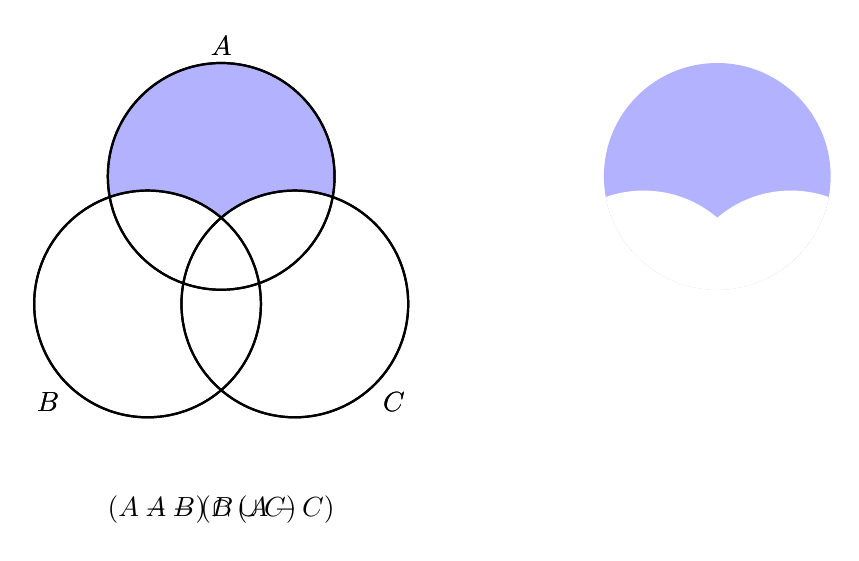
\begin{tikzpicture}[scale=0.9]
    % Left diagram: A - (B \cup C)
    \begin{scope}[shift={(0,0)}]
        \clip (90:1.2) circle (1.6);
        \fill[blue!30] (-4,-4) rectangle (4,4);
        \fill[white] (210:1.2) circle (1.6);
        \fill[white] (330:1.2) circle (1.6);
    \end{scope}
    \draw[thick] (90:1.2) circle (1.6) node[above=1.4cm] {$A$};
    \draw[thick] (210:1.2) circle (1.6) node[below left=1.4cm] {$B$};
    \draw[thick] (330:1.2) circle (1.6) node[below right=1.4cm] {$C$};
    \node at (0, -3.5) {$A - (B \cup C)$};
    
    % Right diagram: (A - B) \cap (A - C)
    \begin{scope}[shift={(7,0)}]
        \clip (90:1.2) circle (1.6);
        \fill[blue!30] (-4,-4) rectangle (4,4);
        \fill[white] (210:1.2) circle (1.6);
        \fill[white] (330:1.2) circle (1.6);
    \end{scope}
    \draw[thick] (90:1.2) circle (1.6) node[above=1.4cm] {$A$};
    \draw[thick] (210:1.2) circle (1.6) node[below left=1.4cm] {$B$};
    \draw[thick] (330:1.2) circle (1.6) node[below right=1.4cm] {$C$};
    \node at (0, -3.5) {$(A - B) \cap (A - C)$};
\end{tikzpicture}
\end{center}

\newpage
\section{Part 5: Conceptual Synthesis and The "Big Picture"}

\subsection{A) Thematic Connections}
The core unifier of this chapter is the concept of \textbf{Algebraic Isomorphism}. You are learning that completely distinct mathematical spaces—sentences of English logic ("and", "or"), electronic boolean circuits (AND gates, XOR gates), and static geometric sets—all obey the exact same underlying mathematical ring structure. De Morgan's Law is not just a rule for sets; it is an omnipresent law of the universe governing how "inverses" interact with "aggregations".

\subsection{B) Forward and Backward Links}
\begin{itemize}
    \item \textbf{Backward Link:} This chapter mathematically formalizes the intuitive Venn diagrams learned in primary arithmetic into a rigorous predicate-logic framework. 
    \item \textbf{Forward Link:} This topic is the unconditional bedrock of \textbf{Measure Theory} and \textbf{Topology}. To formally define a continuous function or calculate the probability of a continuous random variable, one must manipulate infinite, countable unions and intersections of sets ($\sigma$-algebras). If you cannot manipulate 3 sets algebraically here, it is impossible to evaluate $\bigcup_{i=1}^{\infty} A_i$ in real analysis.
\end{itemize}

\section{Part 6: Abstract Real-World Modeling (AI, ML, \& Quant Finance)}

Abstract set operations are directly deployed in the foundational formulation of advanced stochastic models in finance and machine learning.

\subsection{Concrete Scenarios}
\begin{enumerate}
    \item \textbf{Decision Tree Partitions (Machine Learning):} An AI decision tree algorithm splits a universal feature space $\Omega$ (e.g., all patient medical records) into mutually exclusive and exhaustive subsets $A_1, A_2, \dots A_n$ such that $A_i \cap A_j = \emptyset$ and $\bigcup A_i = \Omega$. 
    \item \textbf{Filtrations in Stochastic Calculus (Quant Finance):} In pricing derivative securities (like European Options), the flow of market information over time $t$ is modeled as an increasing sequence of $\sigma$-algebras (sets of sets) denoted as $\mathcal{F}_t$.
\end{enumerate}

\subsection{Mathematical Model Setup: Probability Spaces and Stopping Times}
We formulate a quantitative finance model for an exotic ``Knock-Out Barrier Option''.
Let $(\Omega, \mathcal{F}, \mathbb{P})$ be a probability space representing all possible continuous future market trajectories. The sample space $\Omega$ contains all paths $\omega(t)$ representing the stock price $S_t(\omega)$.

To avoid peeking into the future, we restrict our knowledge to a \textit{filtration} $\{\mathcal{F}_t\}_{t \ge 0}$, where $\mathcal{F}_t$ contains all sets (events) verifiable by time $t$. We define a stopping time $\tau$ (the moment the stock breaches a catastrophic barrier $H$). To ensure $\tau$ is a mathematically valid, predictable event within our set-theory space, the event $\{\tau \le t\}$ must belong to $\mathcal{F}_t$. 

By utilizing the extended distributive and intersection laws from this chapter, we mathematically construct the breach event via an infinite sequence of set intersections and unions over rational time increments $\mathbb{Q}$:
\[ \{\tau \le t\} = \bigcap_{n=1}^\infty \bigcup_{s \in \mathbb{Q} \cap [0, t]} \left\{ \omega \in \Omega \mid S_s(\omega) > H - \frac{1}{n} \right\} \]
This explicitly proves that without the rigorous set operations established via De Morgan's laws and intersections, we could not mathematically define when a financial derivative defaults! 

\newpage
\section{Part 7: Common Variations and Untested Concepts}

A standard university curriculum always includes the \textbf{Symmetric Difference}, an operation critically missing from the provided homework assignment. The Symmetric Difference represents the logical "Exclusive OR" (XOR) operation.

\begin{definition}
The symmetric difference between sets $A$ and $B$, denoted $A \oplus B$ (or $A \Delta B$), is the set of elements in $A$ or $B$, but \textit{not both}.
\[ A \oplus B = (A - B) \cup (B - A) \]
\end{definition}

\begin{theorem}
Prove that $A \oplus B = (A \cup B) - (A \cap B)$.
\end{theorem}
\begin{proof}[Algebraic Proof]
By definition of set difference, $(X - Y) = X \cap \overline{Y}$.
\begin{align*}
(A - B) \cup (B - A) &= (A \cap \overline{B}) \cup (B \cap \overline{A}) \quad &\text{(Definition of Difference)} \\
&= \left[ (A \cap \overline{B}) \cup B \right] \cap \left[ (A \cap \overline{B}) \cup \overline{A} \right] \quad &\text{(Distributive Law)} \\
&= \left[ (A \cup B) \cap (\overline{B} \cup B) \right] \cap \left[ (A \cup \overline{A}) \cap (\overline{B} \cup \overline{A}) \right] \quad &\text{(Distributive Law applied twice)}
\end{align*}
Notice that $X \cup \overline{X} = U$ (the Universal Set), and intersecting any set $Y$ with $U$ is just $Y$.
\begin{align*}
&= \left[ (A \cup B) \cap U \right] \cap \left[ U \cap (\overline{B} \cup \overline{A}) \right] \\
&= (A \cup B) \cap (\overline{B} \cup \overline{A}) \quad &\text{(Identity Law)} \\
&= (A \cup B) \cap \overline{(B \cap A)} \quad &\text{(De Morgan's Law)} \\
&= (A \cup B) - (A \cap B) \quad &\text{(Definition of Difference)}
\end{align*}
The equivalence is rigorously established.
\end{proof}

\section{Part 8: Advanced Diagnostic Testing: "Find the Flaw"}

Below are five exceptionally convincing, yet flawed proofs. Your task is to play the grader, identify the subtle logical error, and correct it.

\begin{problem}[Diagnostic 1]
\textbf{Proposition:} $A - (B \cup C) = (A - B) \cup (A - C)$.
\begin{proof}[Flawed Proof]
Let $x \in A - (B \cup C)$. By definition, $x \in A$ and $x \notin (B \cup C)$. This translates to $x \in A \land (x \notin B \lor x \notin C)$. Distributing the "AND" operation over the "OR" operation yields: $(x \in A \land x \notin B) \lor (x \in A \land x \notin C)$. By definition of set difference, $x \in (A - B) \lor x \in (A - C)$. Therefore, $x \in (A - B) \cup (A - C)$.
\end{proof}
\end{problem}

\begin{problem}[Diagnostic 2]
\textbf{Proposition (The Cancellation Law):} If $A \cup B = A \cup C$, then $B = C$.
\begin{proof}[Flawed Proof]
Assume $A \cup B = A \cup C$. Let $x \in B$. If $x \in A$, then $x \in A \cup C$. If $x \notin A$, then since $x \in B$, it remains true that $x \in A \cup B$. Since $A \cup B = A \cup C$, we deduce $x \in A \cup C$. Because we assumed $x \notin A$, the only way for $x$ to be in $A \cup C$ is if $x \in C$. Thus $B \subseteq C$. By symmetry, $C \subseteq B$, meaning $B = C$.
\end{proof}
\end{problem}

\begin{problem}[Diagnostic 3]
\textbf{Proposition:} The power set of a union is the union of the power sets: $\mathcal{P}(A \cup B) = \mathcal{P}(A) \cup \mathcal{P}(B)$.
\begin{proof}[Flawed Proof]
Let $X \in \mathcal{P}(A \cup B)$. By definition of the power set, $X \subseteq A \cup B$. This means for all elements $x \in X$, $x \in A \cup B$. Hence, $x \in A$ or $x \in B$. This implies that the set $X$ is a subset of $A$ or $X$ is a subset of $B$. Therefore, $X \in \mathcal{P}(A)$ or $X \in \mathcal{P}(B)$, which confirms $X \in \mathcal{P}(A) \cup \mathcal{P}(B)$.
\end{proof}
\end{problem}

\begin{problem}[Diagnostic 4]
\textbf{Proposition:} $(A \cup B) - (A \cap B) = \emptyset$.
\begin{proof}[Flawed Proof]
We use algebra. $(A \cup B) - (A \cap B) = (A \cup B) \cap \overline{(A \cap B)}$. Applying De Morgan's Law yields $(A \cup B) \cap (\overline{A} \cup \overline{B})$. By the Distributive Law, this expands to $(A \cap \overline{A}) \cup (B \cap \overline{B})$. A set intersected with its complement is the empty set $\emptyset$. Thus, we have $\emptyset \cup \emptyset = \emptyset$. 
\end{proof}
\end{problem}

\begin{problem}[Diagnostic 5]
\textbf{Proposition:} If the Cartesian product $A \times B = \emptyset$, then $A = \emptyset$ and $B = \emptyset$.
\begin{proof}[Flawed Proof]
We prove this by contrapositive. Assume it is false that ($A = \emptyset$ and $B = \emptyset$). This assumption means $A \neq \emptyset$ and $B \neq \emptyset$. Therefore, there exists at least one element $a \in A$ and one element $b \in B$. By the definition of the Cartesian product, the coordinate pair $(a, b)$ must exist in $A \times B$. Hence, $A \times B \neq \emptyset$. The contrapositive holds, thus the original proposition is true.
\end{proof}
\end{problem}

\vspace{0.5cm}
\hrule
\vspace{0.5cm}

\subsection{Solution Key (Diagnostic Resolutions)}
\begin{itemize}
    \item \textbf{Resolution 1:} The flaw occurs when negating $x \in (B \cup C)$. The logical negation of $(x \in B \lor x \in C)$ is strictly $(x \notin B \land x \notin C)$ via De Morgan's. The proof hallucinates an "$\lor$" symbol, forcing the false conclusion. The true operation is $(A - B) \cap (A - C)$.
    \item \textbf{Resolution 2:} The flaw is in the first case: "If $x \in A$, then $x \in A \cup C$." While true, this \textit{does not} prove that $x \in C$. For example, if $A = \{1\}, B = \{1\}, C = \emptyset$, then $A \cup B = A \cup C = \{1\}$, but $B \neq C$. The cancellation law is a hallucinated algebraic fallacy.
    \item \textbf{Resolution 3:} The flaw is in deducing ``$X \subseteq A$ or $X \subseteq B$'' from ``for all $x \in X, x \in A$ or $x \in B$.'' The subset $X$ could contain one element from $A$ and a completely different element from $B$, meaning it is a subset of neither individually! (e.g., $A=\{1\}, B=\{2\}, X=\{1,2\}$). 
    \item \textbf{Resolution 4:} The algebraic FOIL (distribution) step is entirely flawed. $(A \cup B) \cap (\overline{A} \cup \overline{B})$ does not expand to just two terms. It correctly expands to $(A \cap \overline{A}) \cup (A \cap \overline{B}) \cup (B \cap \overline{A}) \cup (B \cap \overline{B})$. While the first and last terms are indeed $\emptyset$, the middle two evaluate to $(A - B) \cup (B - A)$, which is the non-empty Symmetric Difference.
    \item \textbf{Resolution 5:} The flaw is a critical failure in propositional logic. The negation of the statement ``($A = \emptyset \land B = \emptyset$)'' is strictly ``($A \neq \emptyset \lor B \neq \emptyset$)''. The proof treats the negation as an AND operator, which restricts the universe. If $A=\{1\}$ and $B=\emptyset$, $A \times B$ is still empty, rendering the original proposition false. 
\end{itemize}

\end{document}